\documentclass[11pt]{article}
\usepackage{latexsym}
\usepackage{amsmath}
\usepackage{amssymb}
\usepackage{amsthm}
\usepackage{epsfig}
\usepackage{graphicx}
\usepackage[tight]{subfigure}
% \usepackage{subcaption}
\usepackage{hyperref}

\usepackage{amsmath}
\usepackage{bbm}

\DeclareMathOperator*{\minimize}{min}
\DeclareMathOperator*{\maximize}{max}
\DeclareMathOperator*{\argmax}{arg\,max}
\DeclareMathOperator*{\argmin}{arg\,min}

\def\RR{\mathbb{R}}
\def\BB{\mathbb{B}}
\def\AA{\mathbb{A}}
\def\PP{\mathbb{P}}
\def\EE{\mathbb{E}}
\def\FF{\mathbb{F}}
\def\HH{\mathcal{H}}
\def\XX{\mathcal{X}}
\def\YY{\mathcal{Y}}
\def\NN{\mathbb{N}}
\def\TT{\mathcal{T}}
\def\DD{\mathcal{D}}
\def\SS{\mathcal{S}}
\def\LL{\mathcal{L}}
\def\MM{\mathcal{M}}
\def\err{\text{err}}
\def\ind{\mathbbm{1}}
\def\II{\mathcal{I}}
\def\ig{\mathcal{\gemini}}
\def\Lev{\textscl}



\usepackage{algorithm}
 %on linux you may need to run sudo apt-get install texlive-full to install algorithm.sys
\usepackage{algorithmic}

\usepackage{verbatim}

\newcommand{\handout}[5]{
  \noindent
  \begin{center}
  \framebox{
    \vbox{
      \hbox to 5.78in { {#1} \hfill #2 }
      \vspace{4mm}
      \hbox to 5.78in { {\Large \hfill #5  \hfill} }
      \vspace{2mm}
      \hbox to 5.78in { {\em #3 \hfill #4} }
    }
  }
  \end{center}
  \vspace*{4mm}
}

\newcommand{\lecture}[5]{\handout{#1}{#2}{#3}{#4}{#5}}
\newcommand{\collision}[0]{\mathrm{collision}}
\newcommand{\nocollision}[0]{\overline{\collision}}

\newcommand*{\QED}{\hfill\ensuremath{\square}}

\newtheorem{theorem}{Theorem}
\newtheorem{corollary}[theorem]{Corollary}
\newtheorem{lemma}[theorem]{Lemma}
\newtheorem{observation}[theorem]{Observation}
\newtheorem{proposition}[theorem]{Proposition}
\newtheorem{definition}[theorem]{Definition}
\newtheorem{claim}[theorem]{Claim}
\newtheorem{fact}[theorem]{Fact}
\newtheorem{assumption}[theorem]{Assumption}
\newtheorem{note}[theorem]{Note}

% 1-inch margins, from fullpage.sty by H.Partl, Version 2, Dec. 15, 1988.
\topmargin 0pt
\advance \topmargin by -\headheight
\advance \topmargin by -\headsep
\textheight 8.9in
\oddsidemargin 0pt
\evensidemargin \oddsidemargin
\marginparwidth 0.5in
\textwidth 6.5in

\parindent 0in
\parskip 1.5ex
%\renewcommand{\baselinestretch}{1.25}

\begin{document}

\lecture{Statistical Techniques in Robotics (16-831, S22)}{Lecture \#16
  (Monday, March 21, 2022)}{Lecturer: Kris Kitani}{Scribe: Michelle Zhao}{Model-Free Value Prediction}

\section{Review}
\subsection{Markov Decision Process}
A Markov Decision Process (MDP) defines a fully observable environment where outcomes are partly random and partly determined by the control of a decision-making agent. $\SS$ is the set of states. $\AA$ defined the set of actions available to the agent. The transition function $p(s'|s,a)$ determines how the state changes based on a action taken by the agent. $r: \SS \rightarrow \RR$ is the reward function. The agent's policy is denoted $\pi: \SS \rightarrow \AA$. 

\subsection{Reinforcement Learning Objective}
The objective in reinforcement learning is to train a policy, or decision-making algorithm, to learn optimal behavior in some environment. In Reinforcement Learning (RL), algorithms interact with an environment, $E$, to learn a policy, $\pi$, which determines a state to action mapping of learned behavior. In each interaction with the environment, the RL agent observes a state of the environment $s$. The agent policy $\pi$ determines an action to take $a$. Upon taking action $a$, the environment returns a reward $r$ to the agent, and transitions to the next state $s'$, which serves as the next input into the agent policy. The agent's aim is to maximize its total reward received.

\begin{figure}[H]
    \centering
    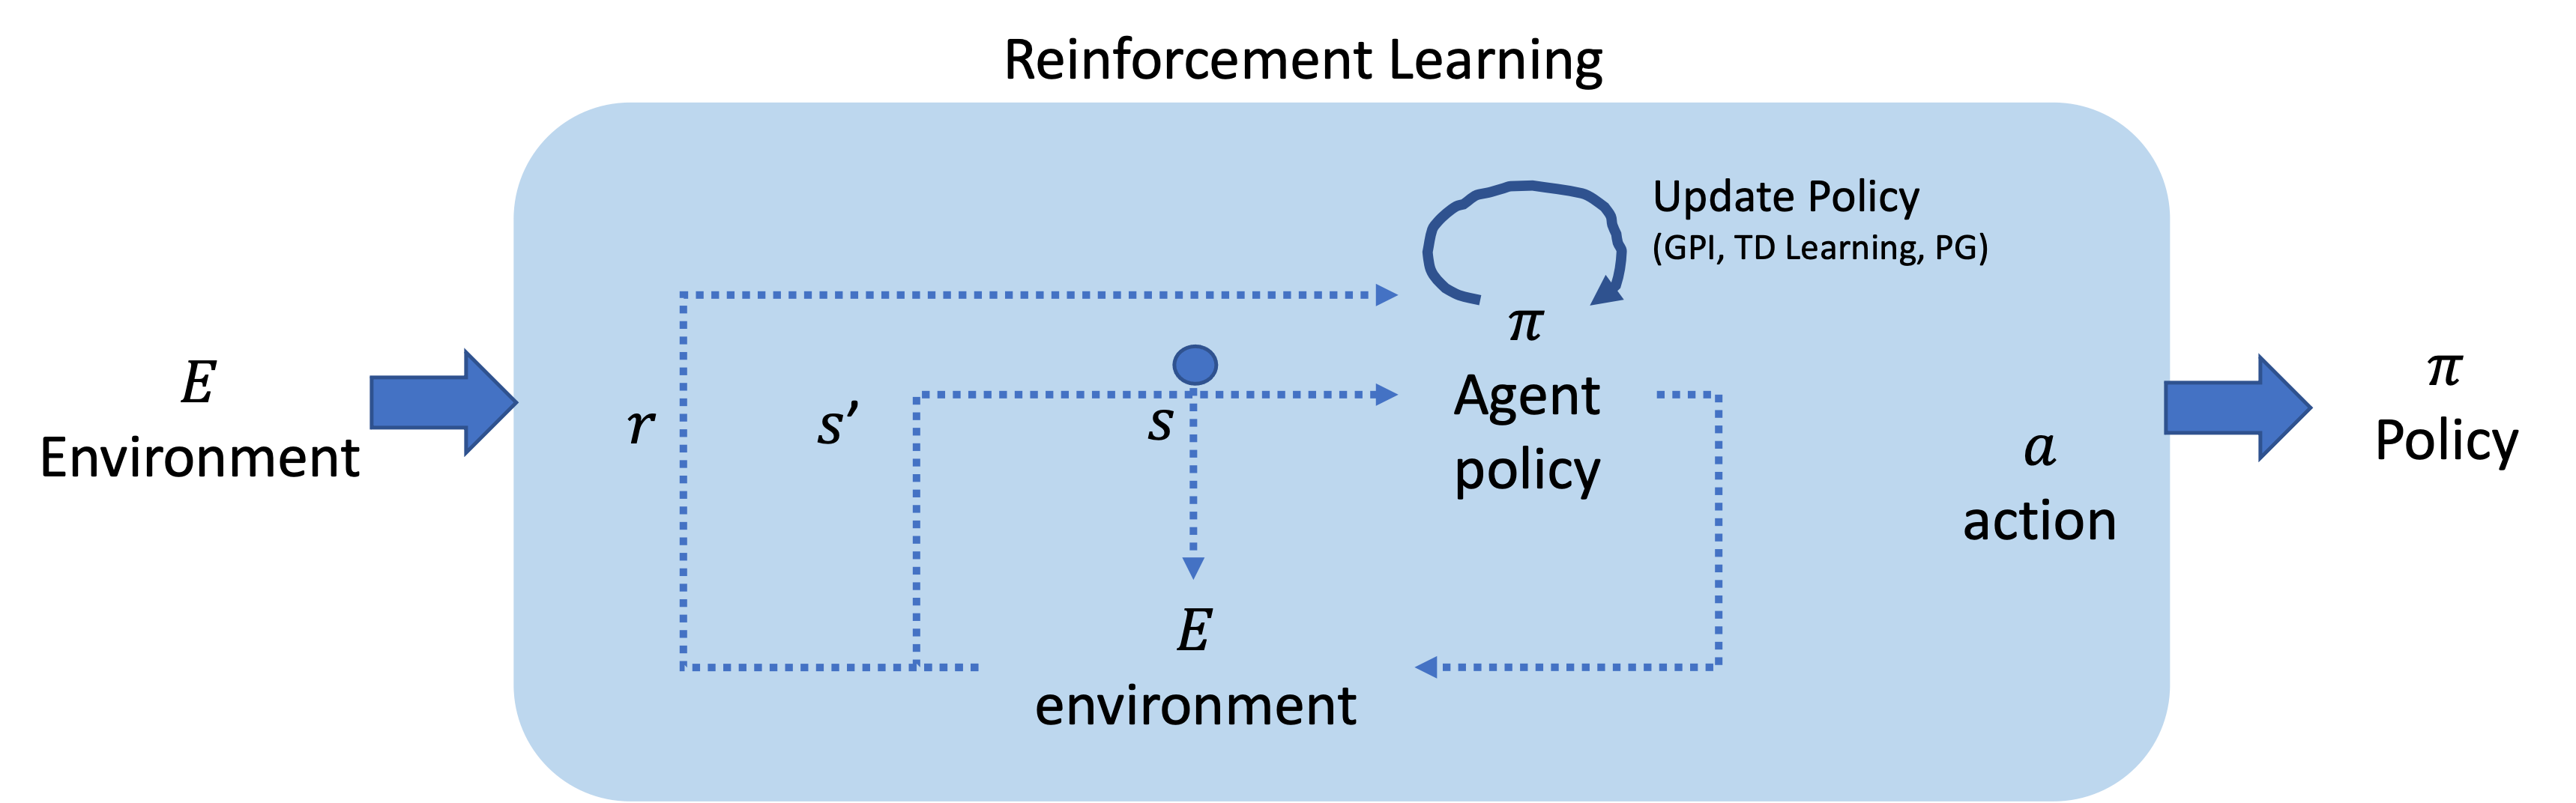
\includegraphics[width=0.8\textwidth]{images/rl_basic.png}
    \caption{Reinforcement learning loop}
    \label{fig:rl_loop}
\end{figure}

\subsection{Reinforcement Learning Approaches}
RL approaches can be broken down into three categories of methods: (1) Policy-based, (2) Value-based, and (3) Hybrid. 
\begin{itemize}
    \item Policy-based: In Policy-based methods, the agent maintains an explicit policy representation that maps state to action $\pi: s \rightarrow a$. Examples of policy representations include neural networks. 
    \item Value-based: In Value-based RL, the agent does not maintain an explicit policy function. Instead, it stores a state value function, representing expected reward in different states, or a state-action value function, representing expected reward for different actions in different states. The agent then acts according to the action with the highest state-action value. An example of a value-based approach is value iteration. 
    \item Hybrid: Hybrid approaches incorporate both policy-based and value-based approaches, modeling both the value function and policy function. An example of hybrid approaches are actor-critic methods.
\end{itemize}

\subsection{Value Based Control}
\begin{figure}[H]
    \centering
    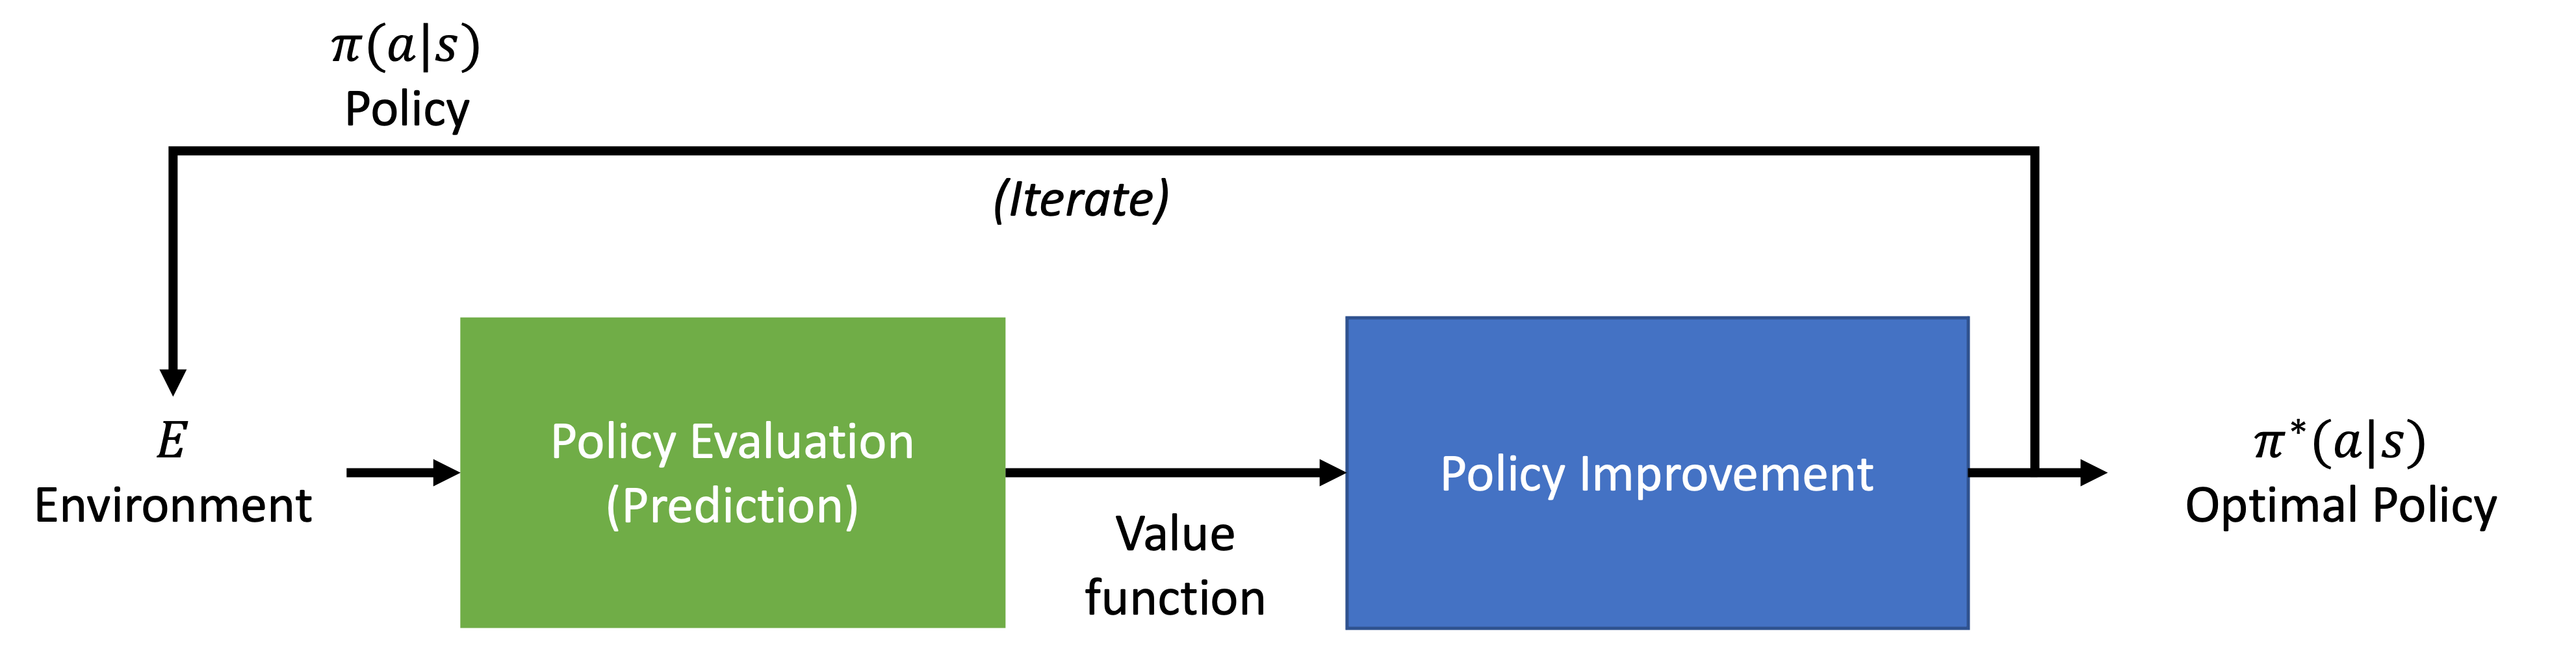
\includegraphics[width=0.8\textwidth]{images/value_based_control.png}
    \caption{Value-based Control}
    \label{fig:vbc}
\end{figure}

In value-based control, an explicit value function is used to select actions. The last lecture introduced Policy Iteration and Value Iteration, two value-based control algorithms, defined below. In Policy Iteration, the first step is policy evaluation, otherwise known as the prediction step. In the policy evaluation step: the agent takes in some state of the environment and outputs a value function: the Q-values for each state-action. What makes this value-based control is that the agent maintains an explicit estimation of the value function. In the second step, the agent improves the policy, by taking an arg-max over actions under the new Q-values, $\pi(a|s) \leftarrow \argmax_a Q(s,a) \forall s$. 

\begin{algorithm}[H]
\caption{Policy Iteration}
\label{algo:PI}
\begin{algorithmic}[1]
\STATE $V \leftarrow rand(\RR)$ \hfill
\STATE $V' \leftarrow rand(\RR)$ \hfill
\WHILE{$\max_a |V(s) - V'(s)| \geq \epsilon$} 
\STATE $V' \rightarrow V$ \hfill
\FOR{$s \in S$}

\STATE $Q(s,a) = r(s) + \gamma \sum_{s'} p(s'|s,a)V'(s')$ \hfill 
% \STATE $\pi(s) = \argmax_a Q(s,a)$ \hfill
\STATE $V(s) = \sum_a \pi(a|s) Q(s,a)$  \hfill

\ENDFOR
\ENDWHILE

\FOR{$s \in S$} 

% \STATE $Q(s,a) = r(s) + \gamma \sum_{s'} p(s'|s,a)V'(s')$ \hfill 
\STATE $\pi(s) = \argmax_a Q(s,a)$ \hfill
% \STATE $V(s) = \sum_a \pi(a|s) Q(s,a)$  \hfill

\ENDFOR


\end{algorithmic}
\end{algorithm}


In Value Iteration, the policy and value function are improved in the same loop. The algorithm does not wait for $V$ to converge for a given policy $\pi$ before updating the policy. 
\begin{algorithm}[H]
\caption{Value Iteration}
\label{algo:VI}
\begin{algorithmic}[1]
\STATE $\pi \leftarrow rand(\AA)$ \hfill
\STATE $V \leftarrow rand(\RR)$ \hfill
\STATE $V' \leftarrow rand(\RR)$ \hfill
\WHILE{$\max_a |V(s) - V'(s)| \geq \epsilon$} 
\STATE $V' \rightarrow V$
\FOR{$s \in S$}

\STATE $Q(s,a) = r(s, a) + \gamma \sum_{s'} p(s'|s,a)V(s')$ \hfill 
\STATE $\pi(s) = \argmax_a Q(s,a)$ \hfill
\STATE $V(s) = Q(s,\pi(s))$  \hfill

\ENDFOR
\ENDWHILE
\end{algorithmic}
\end{algorithm}


\section{Model-Based vs Model-Free RL}
There are two ways the agent can receive the environment, which yields two different types of value prediction algorithms. In Model-based RL, the agent has access to a fully-specified model of the environment. This means that agent knows how states transition to other states based on the actions taken. The agent also has access to how rewards are provided in each state based on the actions taken. One example of this is a gridworld environment, where the reward-providing goals, are visible, and the agent knows that actions moving in any direction will take them to the corresponding adjacent cell. 


In the Model-free scenario, the agent is limited with interactions with the environment. The agent does not have direct access to the transition dynamics or reward function, and instead must learn behavior through repeated interactions with the environment. 



\subsection{Model-Based Prediction}

In Model-based prediction, the agent uses the specified model of the environment to compute the value function. We assume access to a fully specified joint state-reward transition model, $p(s', r|s,a)$. Using this specified model, we can derive the state transition dynamics and reward function. The state transition dynamics are computed by marginalizing out the reward $p(s'|s,a) = \sum_r p(s', r|s, a)$. The reward function can then be computed by utilizing the state transition dynamics.
$$\EE_p[r^t|s^{t+1}=s', a^t=a, s^t = s] = \sum_r r\times \frac{p(s'. r|s, a)}{p(s'|s,a)} = r(s', a, s)$$
$$\EE_p[r^t|a^t=a, s^t = s] = \sum_{r, s'} r\times p(s'. r|s, a) = r(s, a)$$


\subsection{Model-Free Prediction}
In model-free RL, nature only provides the learning algorithm with sampled feedback. The agent only has indirect access to the transition and reward dynamics by interacting with the environment. We use interactions with the environment to compute the value function. Repeated interactions with the environment yield multiple samples $$\{s', r, s, a\}_{n=1}^N$$ where $s$ represents the current state, $a$ represents the action taken by the agent, $r$ represents the reward received from the environment upon taking action $a$, and $s'$ represents the next state.

There are 2 ways in which we can compute the value function using sampled interaction with the environment:
\begin{enumerate}
    \item System Identification: The system identification approach makes an approximation of the state transition dynamics and reward function based on repeated interactions. Once the algorithm has estimated the dynamics, it can convert the problem to a model-based prediction problem. 
    \item Model-free prediction: The approach directly estimates the value function based on interactions with the environment. This lecture will focus on Monte-Carlo and N-Step TD methods for model-free prediction.
\end{enumerate}


\begin{figure}[H]
    \centering
    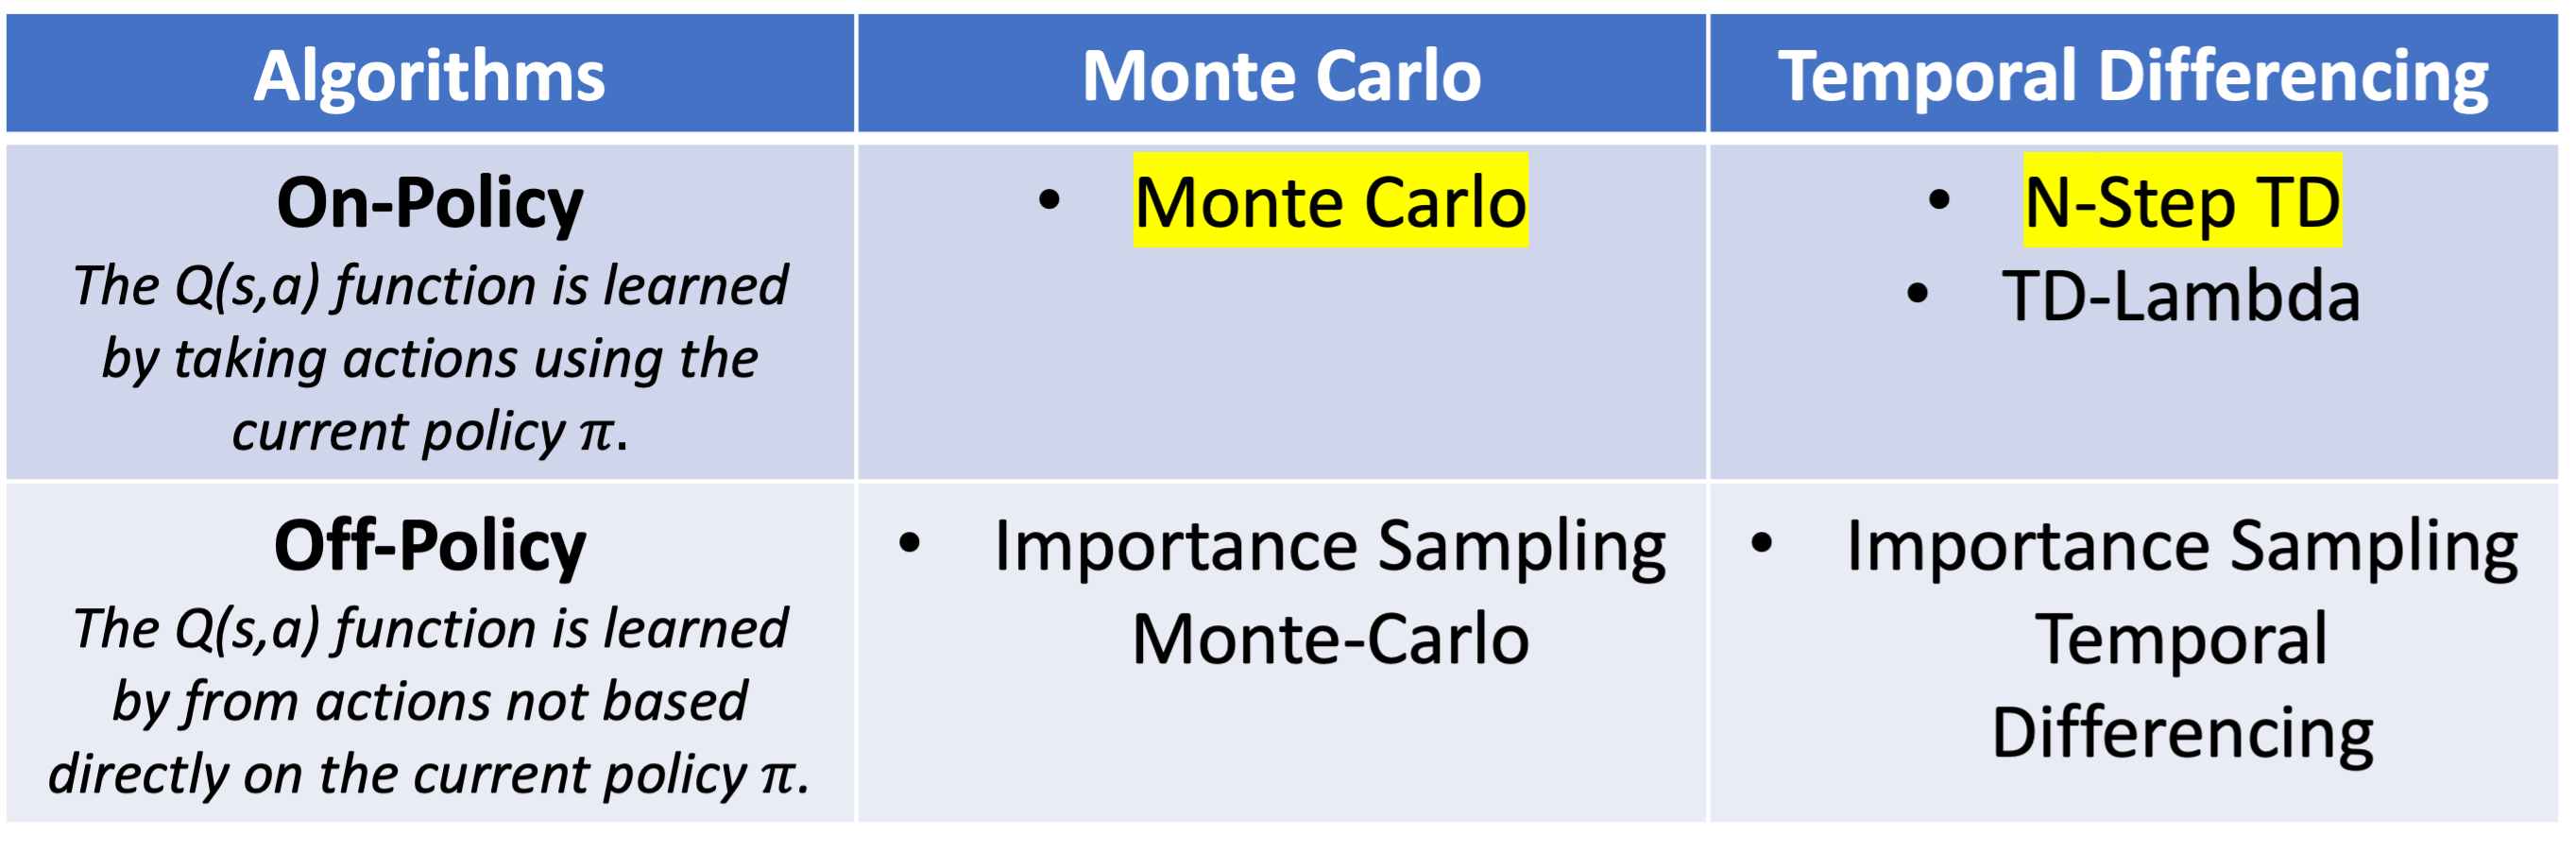
\includegraphics[width=0.6\textwidth]{images/algo_table.png}
    \caption{Model-free prediction methods covered. For context, Deep Q-Learning is an example of a temporal differencing method, and AlphaGo, which uses Monte-Carlo tree-search, is an example of a Monte-Carlo method.}
    \label{fig:methods}
\end{figure}


\section{Monte-Carlo Prediction}
The value of a state is the expected (average) return under the MDP, given the agent policy, state transition dynamics, and initial state distribution. 
$$V^{\pi}(s) = \EE_{\pi, P}[\sum_{t=0}^T \gamma^t r_t|s_0=s]$$
$$V^{\pi}(s) = \EE_{\pi, P}[G|s_0=s]$$
where the return $G = \sum_{t=0}^T \gamma^t r_t$ is the cumulative discounted reward over a single episode.

In a model-free scenario, we cannot compute this expectation because we don't have access to the transition dynamics model. Therefore, we must compute the return by interacting with the environment many times and use the average return as a Monte-Carlo estimate of the value function.
$$V(s) = \frac{1}{N} \sum_{i=1}^N G_i(s)$$
where $N$ is the number of interaction samples, and $G_i(s)$ is the return of state $s$ in interaction $i$.  

We will cover 4 Monte-Carlo prediction algorithms:
\begin{enumerate}
    \item First-Visit MC Prediction
    \item First-Visit Incremental MC Prediction
    \item First-Visit Dynamic MC Prediction
    \item Every-Visit MC Prediction
\end{enumerate}


\subsection{First-Visit MC Prediction}
\begin{algorithm}[H]
\caption{First-Visit MC Prediction $(\pi)$}
\label{algo:FVMC}
\begin{algorithmic}[1]
\STATE $G \leftarrow \mathbf{0}$ \hfill
\FOR{$e = 1,..., E$}

\STATE $\{s^{(t)}, a^{(t)}, r^{(t)}\}_{t=0}^T \sim \varepsilon|\pi$ \hfill 
\FOR{$t = 0,..., T$}
\IF{first visit to state $s^{(t)}$ in episode $e$}
\STATE $G(s^{(t)}) \leftarrow G(s^{(t)}) + \sum_{i=t}^T r^{(i)}$ \hfill 
\STATE $N(s^{(t)}) \leftarrow N(s^{(t)})  + 1$ \hfill 
\ENDIF


\ENDFOR

\ENDFOR

\STATE Return $V(s) \leftarrow \frac{G(s)}{N(s)}$  \hfill
\end{algorithmic}
\end{algorithm}

$E$ represents the number of episodes. For each episode, given some policy $\pi$, the agent can roll-out a trajectory of samples $\{s^{(t)}, a^{(t)}, r^{(t)}\}_{t=0}^T \sim \varepsilon|\pi$ by acting according to policy $\pi$ for $T$ timesteps. Next, we compute the value function by looping over states visited in the interaction sequence. For each state $s^t$ in episode $e$, if it is the first visit to state $s^t$ in the sequence, then the future reward is added to the returns of this state. The counter for visits to this state $N(s)$ is incremented. The policy stays the same for the entire time. The final value function for each state is computed at the end of the algorithm.

\subsection{First-Visit Incremental MC Prediction}
The incremental version of the First-Visit MC Prediction algorithm helps the algorithm generalize to the more common value function update. At every timestep in each episode, if the state $s^t$ in episode $e$ is the first visit to state $s^t$ in the sequence, the return $G(s^{(t)})$ is updated, as well as the value function $V(s)$. 

\begin{algorithm}[H]
\caption{First-Visit Incremental MC Prediction $(\pi)$}
\label{algo:FVIMC}
\begin{algorithmic}[1]
\STATE $V \leftarrow \mathbf{0}$ \hfill
\FOR{$e = 1,..., E$}

\STATE $\{s^{(t)}, a^{(t)}, r^{(t)}\}_{t=0}^T \sim \varepsilon|\pi$ \hfill 
\FOR{$t = 0,..., T$}
\IF{first visit to state $s^{(t)}$ in episode $e$}
\STATE $G(s^{(t)}) \leftarrow \sum_{i=t}^T r^{(i)}$ \hfill 
\STATE $N(s^{(t)}) \leftarrow N(s^{(t)})  + 1$ \hfill 
\STATE $V(s) \leftarrow V(s) + \frac{1}{N(s^{(t)})}(G(s^{(t)})-V(s^{(t)}))$  \hfill
\ENDIF

\ENDFOR
\ENDFOR
\STATE Return $V(s)$  \hfill
\end{algorithmic}
\end{algorithm}

The incremental updates are a weighted average of the return up until the current point and the return the agent has just received. 
$$V(s) = \frac{N(s)-1}{N(s)} V(s) + \frac{1}{N(s)}G_e(s)$$
$$V(s) = V(s) - \frac{1}{N(s)} V(s) + \frac{1}{N(s)}G_e(s)$$
$$V(s) = V(s) - \frac{1}{N(s)} (G_e(s)-V(s))$$


\subsection{First-Visit Dynamic MC Prediction}
The incremental updates are advantageous in that it provides intermediate estimates of the value function, rather than needing to wait for the algorithm to complete to obtain the value function. If the environment is stationary, $1/N(s)$ in an appropriate weighting factor for the value function update. If the environment model is not stationary, it may be advantageous to forget old episodes using a constant factor. An $\alpha$ parameter can be used to control how much we should prioritize recent episodes. Higher values of $\alpha$ give more weight to the most recent episodes. The algorithm does not need to keep track of visits to each state.

\begin{algorithm}[H]
\caption{First-Visit Dynamic MC Prediction $(\pi, \alpha)$}
\label{algo:FVDMC}
\begin{algorithmic}[1]
\STATE $V \leftarrow \mathbf{0}$ \hfill
\FOR{$e = 1,..., E$}

\STATE $\{s^{(t)}, a^{(t)}, r^{(t)}\}_{t=0}^T \sim \varepsilon|\pi$ \hfill 
\FOR{$t = 0,..., T$}
\IF{first visit to state $s^{(t)}$ in episode $e$}
\STATE $G^{(t)} \leftarrow \sum_{i=t}^T r^{(i)}$ \hfill 
\STATE $V(s) \leftarrow V(s) + \alpha(G^{(t)}-V(s^{(t)}))$  \hfill
\ENDIF

\ENDFOR
\ENDFOR
\STATE Return $V(s)$  \hfill
\end{algorithmic}
\end{algorithm}


\subsection{Every-Visit MC Prediction}
In Every-Visit MC Prediction, instead of making updates to the returns and value function when the state is in its first visit in the episode, we update the value function on every visit to each state. Similar to First-Visit Dynamic MC Prediction, the algorithm does not need to keep track of visits to each state.

\begin{algorithm}[H]
\caption{Every-Visit MC Prediction $(\pi, \alpha)$}
\label{algo:EVMC}
\begin{algorithmic}[1]
\STATE $V \leftarrow \mathbf{0}$ \hfill
\FOR{$e = 1,..., E$}

\STATE $\{s^{(t)}, a^{(t)}, r^{(t)}\}_{t=0}^T \sim \varepsilon|\pi$ \hfill 
\FOR{$t = 0,..., T$}
\STATE $G^{(t)} \leftarrow \sum_{i=t}^T r^{(i)}$ \hfill 
\STATE $N(s^{(t)}) \leftarrow N(s^{(t)})  + 1$ \hfill 
\STATE $V(s) \leftarrow V(s) + \alpha(G^{(t)}-V(s^{(t)}))$  \hfill
\ENDFOR
\ENDFOR
\STATE Return $V(s)$  \hfill
\end{algorithmic}
\end{algorithm}

Notes on Every-Visit MC Prediction
\begin{itemize}
    \item Line 5 is inefficient. The algorithm can be optimized for efficiency by iterating backwards from the end of the episode and cache returns. 
    \item Monte Carlo (MC) cannot be used for non-terminating problems (infinite horizon), because MC relies on knowing all returns for an entire episode, thus requiring a terminating episode. 
    \item You can compute the value function after each action is sampled by the policy by estimating returns using an intermediate value function estimate. This is temporal difference learning.
\end{itemize}

\subsection{Properties of MC Prediction}
\begin{itemize}
    \item MC prediction is model-free.
    \item Monte Carlo estimates of return have high variance. When trajectories are short, there isn't as much variance. However, each step incorporates randomness, or stochasticity, which compounds as trajectories get longer, leading to extremely high variance. Thus, MC estimates have high variance due to the compounding factors of long sequences. 
    \item MC prediction works for finite horizon problems.
    \item MC prediction uses full returns (does not use bootstrapping) to estimate the value function, which yields an unbiased (zero-bias) estimate.
    \item MC prediction converges to the MSE (mean-squared error) solution. 
\end{itemize}


\section{Temporal Difference (TD) Prediction}
Temporal Difference (TD) Prediction allows us a way to extend MC prediction for online updates to the value function based on actions taken by the agent policy. It also allows us to extend MC prediction to the continuous learning case (single long episode). Temporal difference prediction learns from raw experience like MC prediction but also introduces the idea of bootstrapping (from dynamic programming) to incrementally update the values after each action. 

MC prediction requires the entire episode to be complete in order to update the value function, and thus can't handle continuous problems. In TD learning, the empirical return can be decomposed into immediate rewards and value function updates.

The Monte-Carlo update equation is 
$$V(s) \leftarrow V(s) + \alpha(G^{(t)}-V(s^{(t)}))$$
The empirical return $G^{(t)}$ can be expanded into 
$$G^{(t)}(1) = r^{(t)} + \gamma V(s^{(t+1)})$$
where $r^{(t)}$ is the immediate reward and $\gamma V(s^{(t+1)})$ is the estimated value. $r^{(t)} + \gamma V(s^{(t+1)})$ represents the 1-step TD target.

The 1-step TD update is:
$$V(s) \leftarrow V(s) + \alpha(r^{(t)} + \gamma V(s^{(t+1)})-V(s^{(t)}))$$
$(r^{(t)} + \gamma V(s^{(t+1)})-V(s^{(t)}))$ represents the 1-step TD error.

The empirical return $G^{(t)}$ can be expanded further into the 2-step TD target:
$$G^{(t)}(2) = r^{(t)} + \gamma r^{(t+1)} + \gamma^2 V(s^{(t+2)})$$
The 2-step TD update is:
$$V(s) \leftarrow V(s) + \alpha(r^{(t)} + \gamma r^{(t+1)} + \gamma^2 V(s^{(t+2)})-V(s^{(t)}))$$
$(r^{(t)} + \gamma r^{(t+1)} + \gamma^2 V(s^{(t+2)})-V(s^{(t)}))$ represents the 2-step TD error.

The N-step TD update is:
$$G^{(t)}(N) = r^{(t)} + \gamma r^{(t+1)}+...\gamma^{N-1} r^{(N-1)}+... + \gamma^N V(s^{(t+N)})$$
$$V(s) \leftarrow V(s) + \alpha(r^{(t)} + \gamma r^{(t+1)}+...\gamma^{N-1} r^{(N-1)}+... + \gamma^N V(s^{(t+N)})-V(s^{(t)}))$$

The infinite-step TD update converges to the Monte-Carlo update:
$$G^{(t)}(\infty) = r^{(t)} + \gamma r^{(t+1)}+...\gamma^{N-1} r^{(N-1)}+... + \gamma^T r^{(T)}$$

\subsection{1-Step TD Prediction}
The key idea of TD prediction is to leave a memo of the value at each state and update the estimate of the state memo value every time the state is visited. 
The one-step TD target does not require access to future rewards.
\begin{algorithm}[H]
\caption{1-Step TD Prediction $(\pi, \alpha)$}
\label{algo:1TD}
\begin{algorithmic}[1]
\STATE $V \leftarrow \mathbf{0}$ \hfill
\FOR{$e = 1,..., E$}

\STATE $\{s^{(t)}, a^{(t)}, r^{(t)}\}_{t=0}^T \sim \varepsilon|\pi$ \hfill 
\FOR{$t = 0,..., T-1$}
\STATE $G^{(t)}(1) \leftarrow r^{(t)}+ \gamma V(s^{(t+1)})$ \hfill 
\STATE $N(s^{(t)}) \leftarrow N(s^{(t)})  + 1$ \hfill 
\STATE $V(s) \leftarrow V(s) + \alpha(G^{(t)}(1)-V(s^{(t)}))$  \hfill
\ENDFOR
\ENDFOR
\STATE Return $V(s)$  \hfill
\end{algorithmic}
\end{algorithm}

\subsection{N-Step TD Prediction}
The key idea of TD prediction is to leave a memo of the value at each state and update the estimate of the state memo value every time the state is visited. 
The one-step TD target does not require access to future rewards.
\begin{algorithm}[H]
\caption{N-Step TD Prediction $(\pi, \alpha, N)$}
\label{algo:NTD}
\begin{algorithmic}[1]
\STATE $V \leftarrow \mathbf{0}$ \hfill
\FOR{$e = 1,..., E$}

\STATE $\{s^{(t)}, a^{(t)}, r^{(t)}\}_{t=0}^T \sim \varepsilon|\pi$ \hfill 
\FOR{$t = 0,..., T-N$}
\STATE $G^{(t)}(N) \leftarrow \sum_{i=t}^{t+N-1} \gamma^{i-t} r^{(i)}+ \gamma^N V(s^{(t+N)})$ \hfill 
\STATE $N(s^{(t)}) \leftarrow N(s^{(t)})  + 1$ \hfill 
\STATE $V(s) \leftarrow V(s) + \alpha(G^{(t)}(N)-V(s^{(t)}))$  \hfill
\ENDFOR
\ENDFOR
\STATE Return $V(s)$  \hfill
\end{algorithmic}
\end{algorithm}

\subsection{Properties of TD Prediction}
\begin{itemize}
    \item The appropriate value for N depends on the problem.
    \item If N is large, the algorithm can be optimized for efficiency by iterating backwards from the end of the episode and caching returns.
    \item TD prediction can be used for non-terminating problems (infinite horizon) because the value function is updated after each action, using bootstrapping.
    \item TD prediction is model-free.
    \item TD prediction uses bootstrapping (guess of a guess) to estimate the value function. Thus, the estimates are biased.
    \item TD value estimates are low variance, due to the sequences being short in length. 
    \item TD prediction converges to the maximum likelihood solution. The expected reward is weighted by the probability of the state transition. 
\end{itemize}


\section{Summary}
In this lecture, we covered Model-Free Value-based Reinforcement Learning. We covered Monte-Carlo and Temporal Differencing prediction. In model-free RL, the agent only has indirect access to the transition and reward dynamics by interacting with the environment. The agent can use interactions with the environment to compute Monte-Carlo estimates of the value function. There are multiple variants of Monte-Carlo prediction. Temporal Difference (TD) Prediction extends MC prediction for online updates to the value function based on actions taken by the agent policy, allowing for the algorithm to handle infinite horizon problems.

% \section{Appendix}
% \subsection{Convergence Speed Comparison of Policy Iteration and Value Iteration}
% Both algorithms are guaranteed to converge to an optimal policy in the end. Yet, the policy iteration algorithm converges within fewer iterations. As a result, the policy iteration is reported to conclude faster than the value iteration algorithm.

\section*{References}
[1] Leslie Kaebling. Value Iteration Notes, 1996. \url{https://www.cs.cmu.edu/afs/cs/project/jair/pub/volume4/kaelbling96a-html/node19.html}

[2] “Artificial Intelligence.” Artificial Intelligence - Foundations of Computational Agents -- 9.5.3 Value Iteration, \url{https://artint.info/html/ArtInt_227.html#:~:text=Value\%20iteration\%20is\%20a\%20method,uses\%20an\%20arbitrary\%20end\%20point.}
%Include your references here. Please cite any resources you found useful.	
%Populate the refs.bib file or list your references manually. Be consistent in formatting!
{
\bibliography{refs}
\bibliographystyle{abbrv}
}

%\section{Appendix}
%This section provides any relevant background material that was not covered in the lectures, but was found to be useful for understanding the material. 
%For example, derivations, theory underlying techniques employed, etc. 

%Additionally, this section can summarizes applications or extensions of these techniques found in the literature. 

\end{document} % Done!


